%%%%%%%% Project report — VISWORD %%%%%%%%%%%%%%%%%
%%%%%%%% Build with: ./build.sh

\documentclass{article}

\usepackage{microtype}
\usepackage{graphicx}
\usepackage{booktabs}
\usepackage{amsmath}
\usepackage[table]{xcolor}
\usepackage{hyperref}

\newcommand{\theHalgorithm}{\arabic{algorithm}}

\usepackage[accepted]{comp547}

\icmltitlerunning{Visual Encoders for Document Retrieval}

% Encoder-family pastel colours, used consistently in tables and figures.
\definecolor{cITC}{HTML}{D9E8F4}    % image-text contrastive
\definecolor{cSSL}{HTML}{E2F0DE}    % image-only self-supervised
\definecolor{cSUP}{HTML}{F8E1DD}    % supervised classification
\definecolor{cRND}{HTML}{ECECEC}    % random init
\definecolor{cFT}{HTML}{FFF1C2}     % fine-tuned (yellowish)

\begin{document}

\twocolumn[
\icmltitle{Can Vision Models Read?\\
Probing Linguistic Structure via JEPA on Text Screenshots}

\icmlsetsymbol{equal}{*}

\begin{icmlauthorlist}
\icmlauthor{Bar\i{}\c{s} Cem Bakay}{to}
\icmlauthor{Halil \.{I}brahim Kanpak}{to}
\end{icmlauthorlist}

\icmlaffiliation{to}{Department of Computer Engineering, Ko\c{c}
University, Istanbul, Turkey}

\icmlcorrespondingauthor{Halil \.{I}brahim Kanpak}{hkanpak21@ku.edu.tr}

\vskip 0.3in
]

\printAffiliationsAndNotice{}

\begin{abstract}
We ask whether vision models acquire linguistic structure when
their training data consists of rendered text. As a probe, we use
retrieval over a 2\,000-page held-out slice of Wikipedia
screenshots: given a $224{\times}224$ crop, identify its source
page. We compare six encoders trained with five distinct
objectives, including a joint-embedding predictive architecture
(I-JEPA) that is the canonical image-only predictive baseline. The
finding is sharp: image--text contrastive encoders (CLIP, SigLIP)
retrieve at R@10 $=$~0.78 and 0.62 zero-shot, while image-only
predictive (I-JEPA), self-supervised contrastive (DINOv2),
supervised classification (ImageNet ViT), and random-init plain ViT
all sit at R@10 $\le 0.058$. I-JEPA in particular scores
\emph{below} random initialisation. Across the six encoders,
mutual-$k$NN alignment with text encoders rank-correlates with
retrieval R@10 at Spearman $\rho = 0.83$ ($p = 0.04$), supporting
the Platonic Representation Hypothesis as the explanatory axis.
Fine-tuning DINOv2 with a SALAD aggregator on 50\,k pages reaches
R@10 $=$~0.915, exceeding zero-shot CLIP, but every fine-tuned
checkpoint exhibits a layout-fingerprint failure mode: erasing the
top 30\,\% of every test image \emph{improves} cross-set transfer
by up to $6.7\times$, indicating the model learns to overweight
the title region rather than read content.
\end{abstract}

\begin{figure*}[t]
\centering
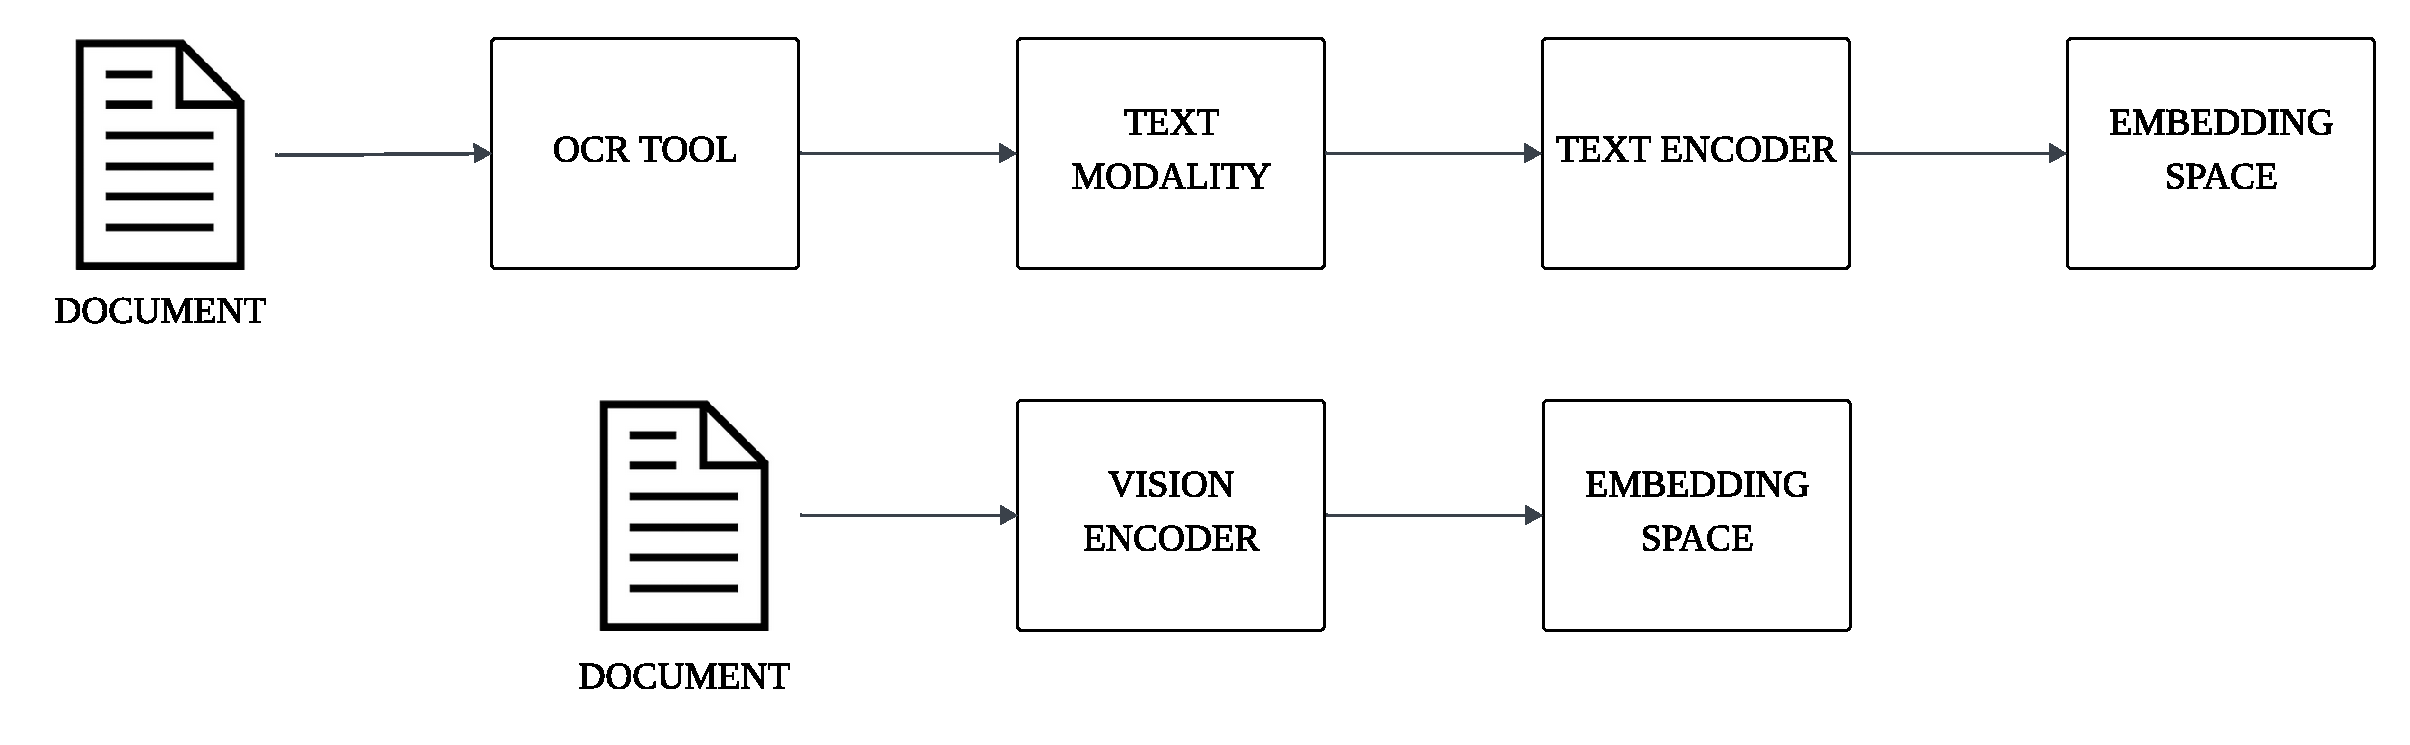
\includegraphics[width=0.9\textwidth]{figures/sysDiagram.pdf}
\caption{The two retrieval paradigms compared in this paper. The
\emph{text} pipeline (top) extracts characters with an OCR tool and
encodes them with a text encoder. The \emph{visual} pipeline
(bottom) feeds the rendered document image directly into a vision
encoder. We study the visual pipeline because it bypasses OCR
errors, multilingual tokeniser failures, and layout discarding,
and because it admits image queries (e.g.\ a crop of an unknown
page) for which no text exists.}
\label{fig:sys}
\end{figure*}

\section{Introduction}
\label{sec:intro}

Documents combine glyph sequences with visual layout. A vision
encoder trained on rendered text could in principle acquire two
distinct kinds of structure: (i)~glyph-level reading (recognising
words and characters as visual patterns), and (ii)~layout-level
structure (titles, infoboxes, lists, figures, captions). The two
pipelines in Figure~\ref{fig:sys} operationalise the alternatives:
the text pipeline OCRs the page and encodes characters; the visual
pipeline encodes the screenshot directly. The visual pipeline is
attractive when text extraction is unreliable (degraded scans,
formula-heavy or multilingual content) or when the query is itself
a visual crop with no text available, but it places the burden of
``reading'' on the encoder.

We probe whether modern vision encoders read in this sense by
measuring how well they retrieve Wikipedia source pages from
$224{\times}224$ crops. The probe is informative because the visual
content \emph{is} the text: an encoder that genuinely reads should
match an encoder that operates on the underlying string. We compare
five families:

\begin{itemize}
\item \textbf{Image--text contrastive} (CLIP, SigLIP) --- learns by
matching images and captions; sees text indirectly.
\item \textbf{Image-only predictive} (I-JEPA) --- the canonical
joint-embedding predictive architecture; trains an image encoder
to predict the latent representations of masked image blocks
\cite{assran2023ijepa}. No text supervision.
\item \textbf{Image-only contrastive} (DINOv2) --- view-contrastive
distillation on natural images. No text supervision.
\item \textbf{Supervised classification} (ImageNet ViT) --- ViT-B/16
trained on ImageNet-21k+1k labels.
\item \textbf{Random initialisation} --- a frozen ViT-B/16 sanity
floor.
\end{itemize}

Three questions:

\textbf{Q1 (zero-shot reading).} Which pretraining produces image
representations from which the source page can be retrieved
zero-shot?

\textbf{Q2 (JEPA specifically).} Does I-JEPA, an image-only
predictive objective with no text supervision, acquire any
linguistic structure detectable through retrieval?

\textbf{Q3 (the Platonic axis).} Does the Platonic Representation
Hypothesis \cite{huh2024platonic} --- which predicts that encoders
trained on diverse objectives converge to a shared abstract
representation --- explain the retrieval ordering quantitatively?
We measure each image encoder's mutual-$k$NN alignment with text
encoders on the same content and ask whether alignment predicts
retrieval performance.

\textbf{Contributions.}
(1)~A leak-free crop$\rightarrow$page protocol with leave-one-out
gallery aggregation.
(2)~A six-encoder zero-shot grid showing image--text contrastive
encoders dominating the four image-only baselines, with I-JEPA
sitting \emph{below} random initialisation.
(3)~A Platonic alignment grid producing the rank correlation
$\rho = 0.83$ between alignment and retrieval, statistically
significant at $n = 6$.
(4)~A reproducible failure mode in every fine-tuned checkpoint:
erasing the top 15--30\,\% of every test image
\emph{improves} cross-set transfer, indicating the model
overweights a layout confound rather than reading content.

\section{Related Work}
\label{sec:related}

\textbf{Pixel-based language models and document AI.} PIXEL
\cite{rust2023pixel}, CLIPPO \cite{tschannen2023clippo} and
Pix2Struct \cite{lee2023pix2struct} all train transformers on
rendered text and demonstrate that pixel inputs can match or exceed
tokenised text on downstream tasks. ColPali
\cite{faysse2025colpali} produces multi-vector page embeddings via
late interaction and shows that direct visual retrieval over
screenshots competes with text+OCR pipelines on the ViDoRe
benchmark. We adopt a simpler single-vector setup to keep our six
encoders comparable on identical infrastructure.

\textbf{Self-supervised vision and post-hoc text alignment.}
DINOv2 \cite{oquab2024dinov2} learns image features via
view-contrastive distillation; I-JEPA \cite{assran2023ijepa} learns
them by predicting masked-block representations. Jose et al.\
\cite{jose2024dinov2text} showed that a small text encoder aligned
post-hoc to a frozen DINOv2 reaches CLIP-level zero-shot
classification, suggesting that self-supervised image features
already contain a linguistically-decodable structure. We test the
analogous claim for I-JEPA on document screenshots.

\textbf{Image--text contrastive pretraining and OCR shortcuts.}
CLIP \cite{radford2021clip} and SigLIP \cite{zhai2023siglip} are
trained contrastively on image--caption pairs, with CLIP using
softmax InfoNCE and SigLIP using a sigmoid pairwise loss. Both
have been shown to read text rendered in images
\cite{materzynska2022spelling, lin2024parrot}; we exploit this in a
title-blanking experiment.

\textbf{Platonic alignment and probing.} Huh et al.\
\cite{huh2024platonic} predict cross-encoder alignment grows with
model and data scale; Maniparambil et al.\
\cite{maniparambil2024crossencoder} and Moayeri et al.\
\cite{moayeri2023text2concept} measure such alignment for
natural-image vision encoders. We extend this measurement to a
document-screenshot domain and use mutual-$k$NN, debiased CKA
\cite{kornblith2019cka, murphy2024align}, and Procrustes distance
on identical 2\,000-page eval slices.

\section{Method}
\label{sec:method}

\subsection{Data and crops}
\label{sec:data}

We use \texttt{Tevatron/wiki-ss-corpus}: $\sim$1.2\,M Wikipedia page
screenshots paired with the page title and rendered body text. We
hold a local cache of $\sim$376\,k pages. A non-overlapping cropper
tiles each page into $490\times490$\,px crops resized to
$224\times224$\,px. At this resolution body text is sub-pixel and
illegible to a ViT patch encoder; only headings and the overall
layout structure remain visually recoverable. ``Reading'' in this
paper therefore refers to heading-level text and visual layout, not
fluent body content.

\begin{figure}[t]
\centering
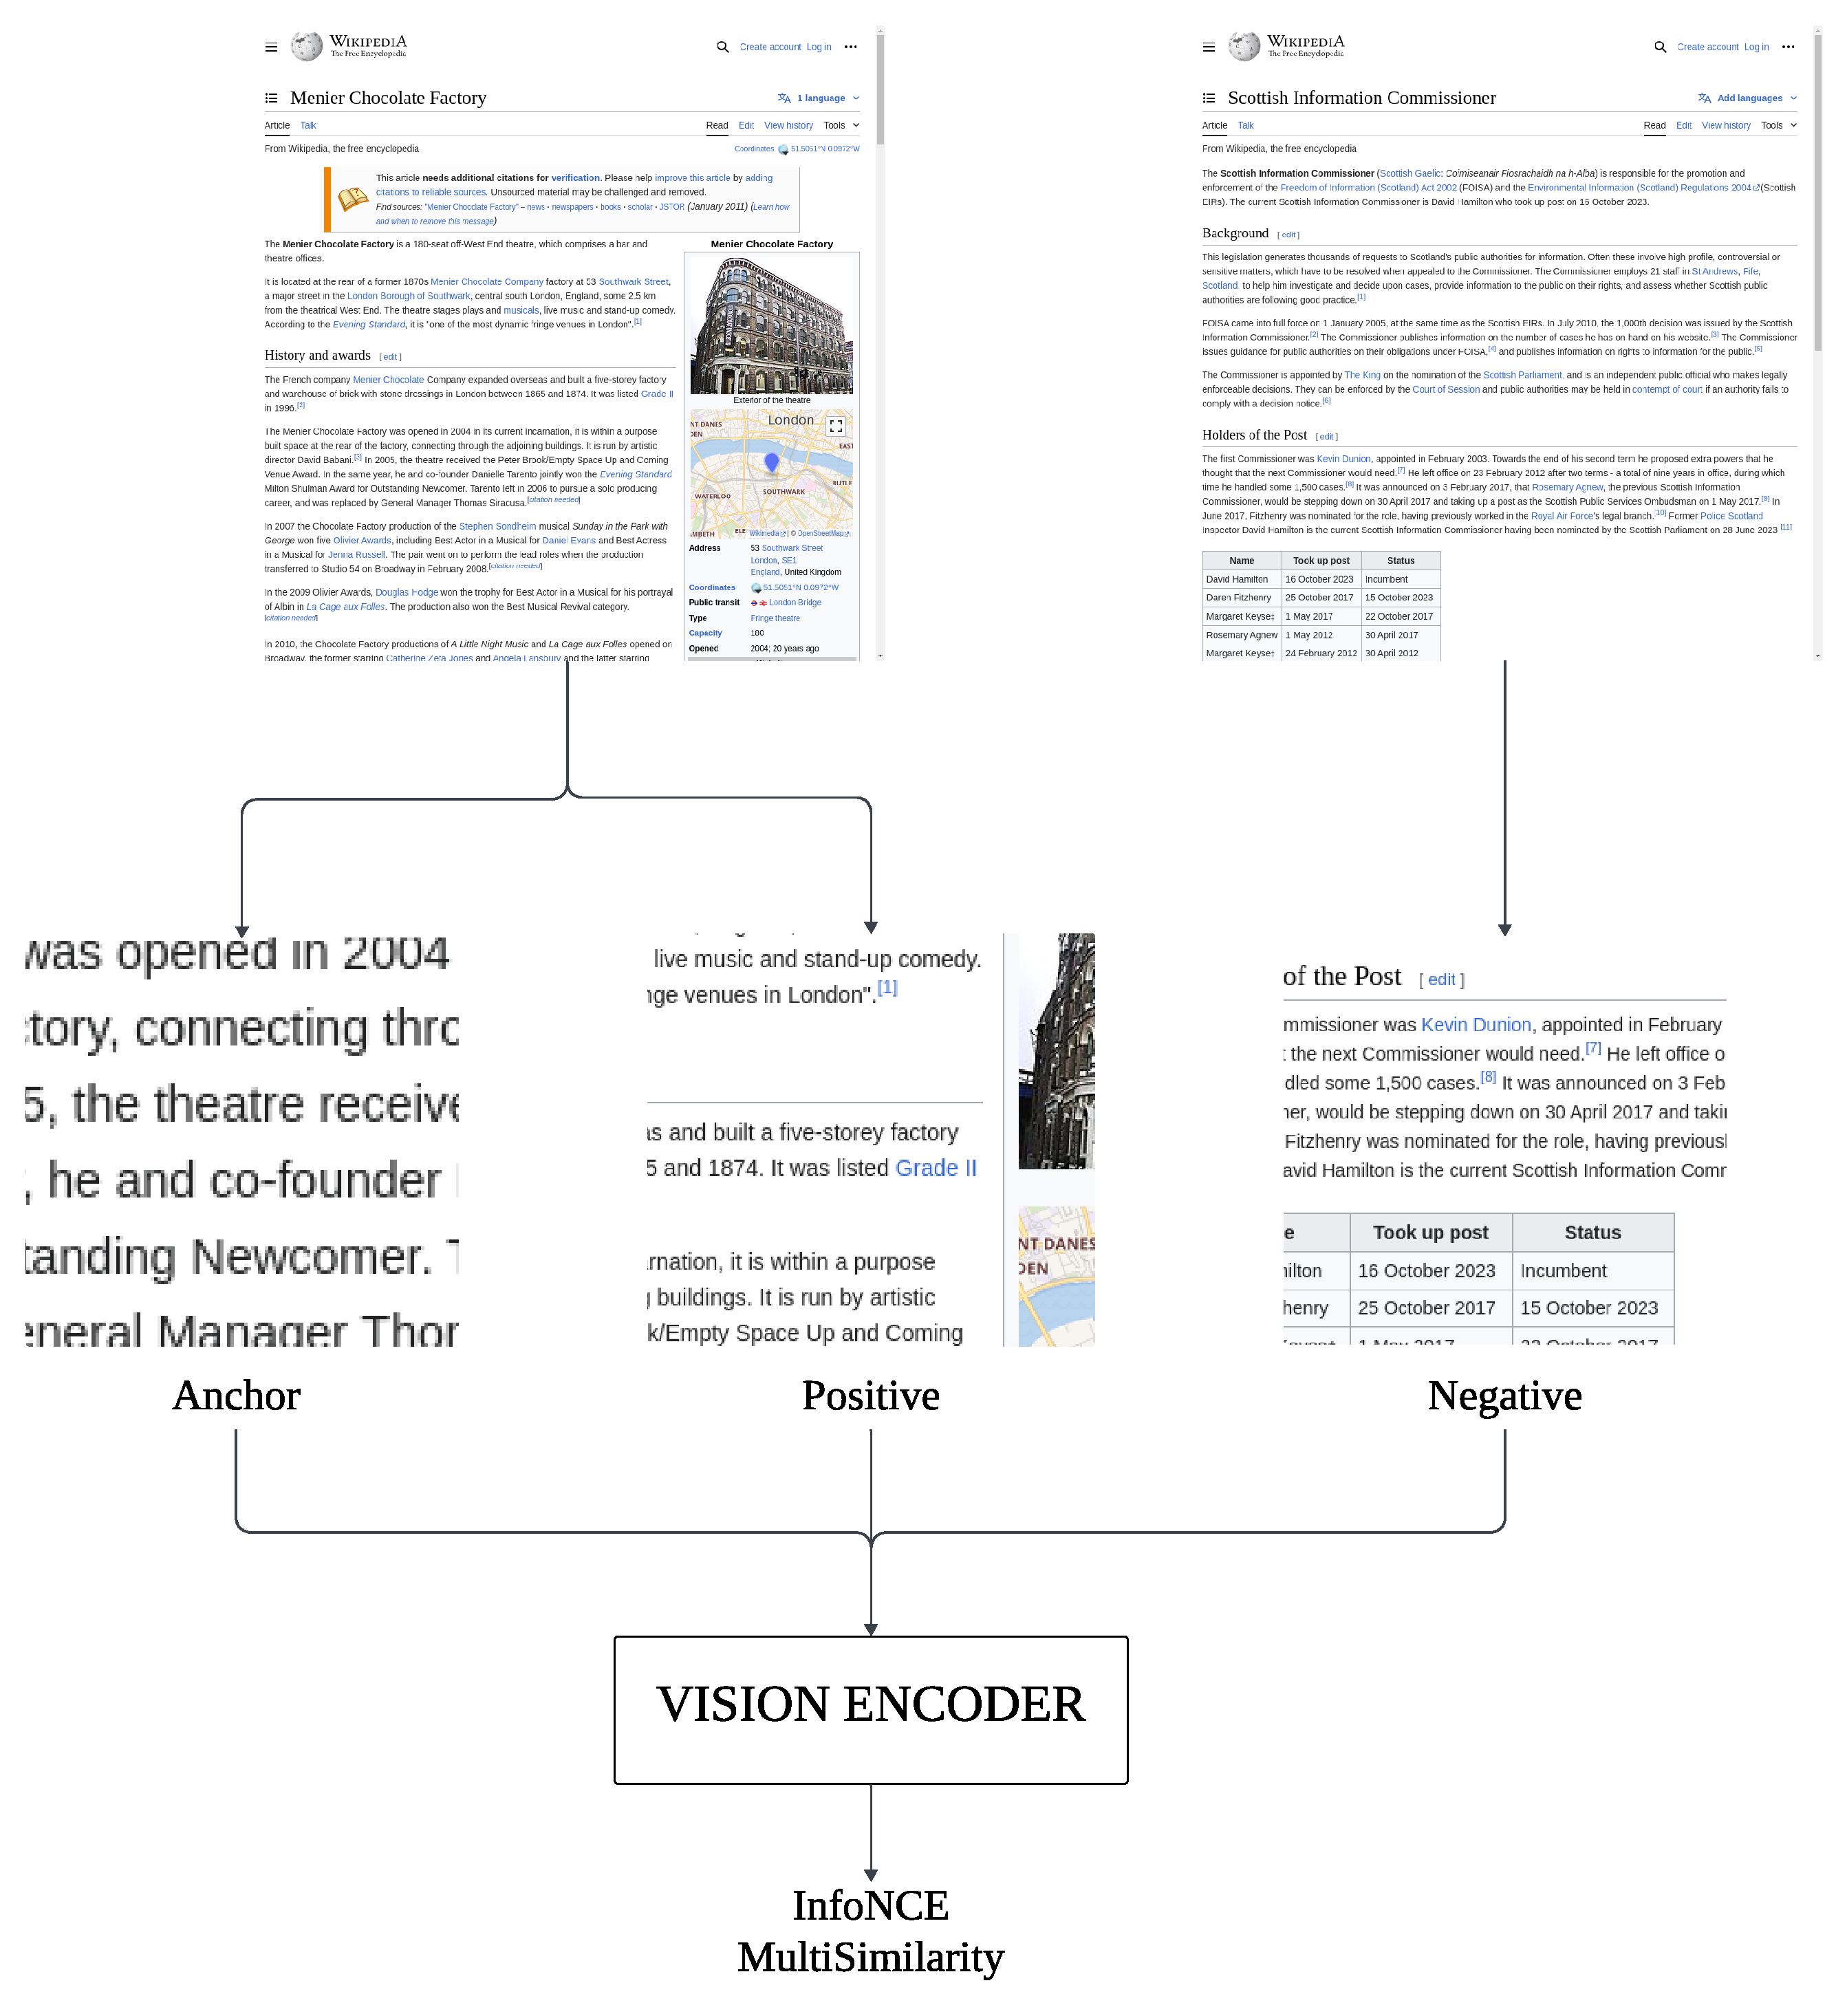
\includegraphics[width=\columnwidth]{figures/Training.pdf}
\caption{Training. Each step samples four pages $\times$ four
crops; same-page crops are positives, cross-page crops are
negatives. The image encoder produces an L2-normalised descriptor;
training minimises a multi-similarity contrastive loss
\cite{wang2019msloss}. We unfreeze the last four ViT blocks
(of twelve) and train a head on top.}
\label{fig:train}
\end{figure}

\subsection{Training (fine-tunes)}
\label{sec:training}

We train each (encoder, head) configuration with the procedure of
Figure~\ref{fig:train}. Each batch contains 4 pages $\times$ 4
crops $=$ 16 images. Within a batch, crops sharing a page are
positives; otherwise negatives. The loss is multi-similarity
\cite{wang2019msloss}. The optimiser is AdamW with weight decay
$10^{-4}$, gradient clip 1.0, linear warmup over 5\,\% of steps
followed by cosine decay. Backbone learning rate is $10^{-5}$ for
DINOv2 and $10^{-7}$ for CLIP and SigLIP (a higher rate causes
catastrophic representation collapse on the latter two), head
learning rate $5\times 10^{-4}$ throughout. Heads are either an
MLP \mbox{($768\to 512\to 256$)} or the SALAD optimal-transport
aggregator \cite{izquierdo2024salad} producing an 8\,448-d
descriptor. Only the head and the last four ViT blocks are
trainable. Fine-tunes use 30\,000 training pages $\times$ 3 epochs
(5\,625 optimiser steps), one seed; the saturation
diagnostic uses 50\,000 pages.

\begin{figure}[t]
\centering
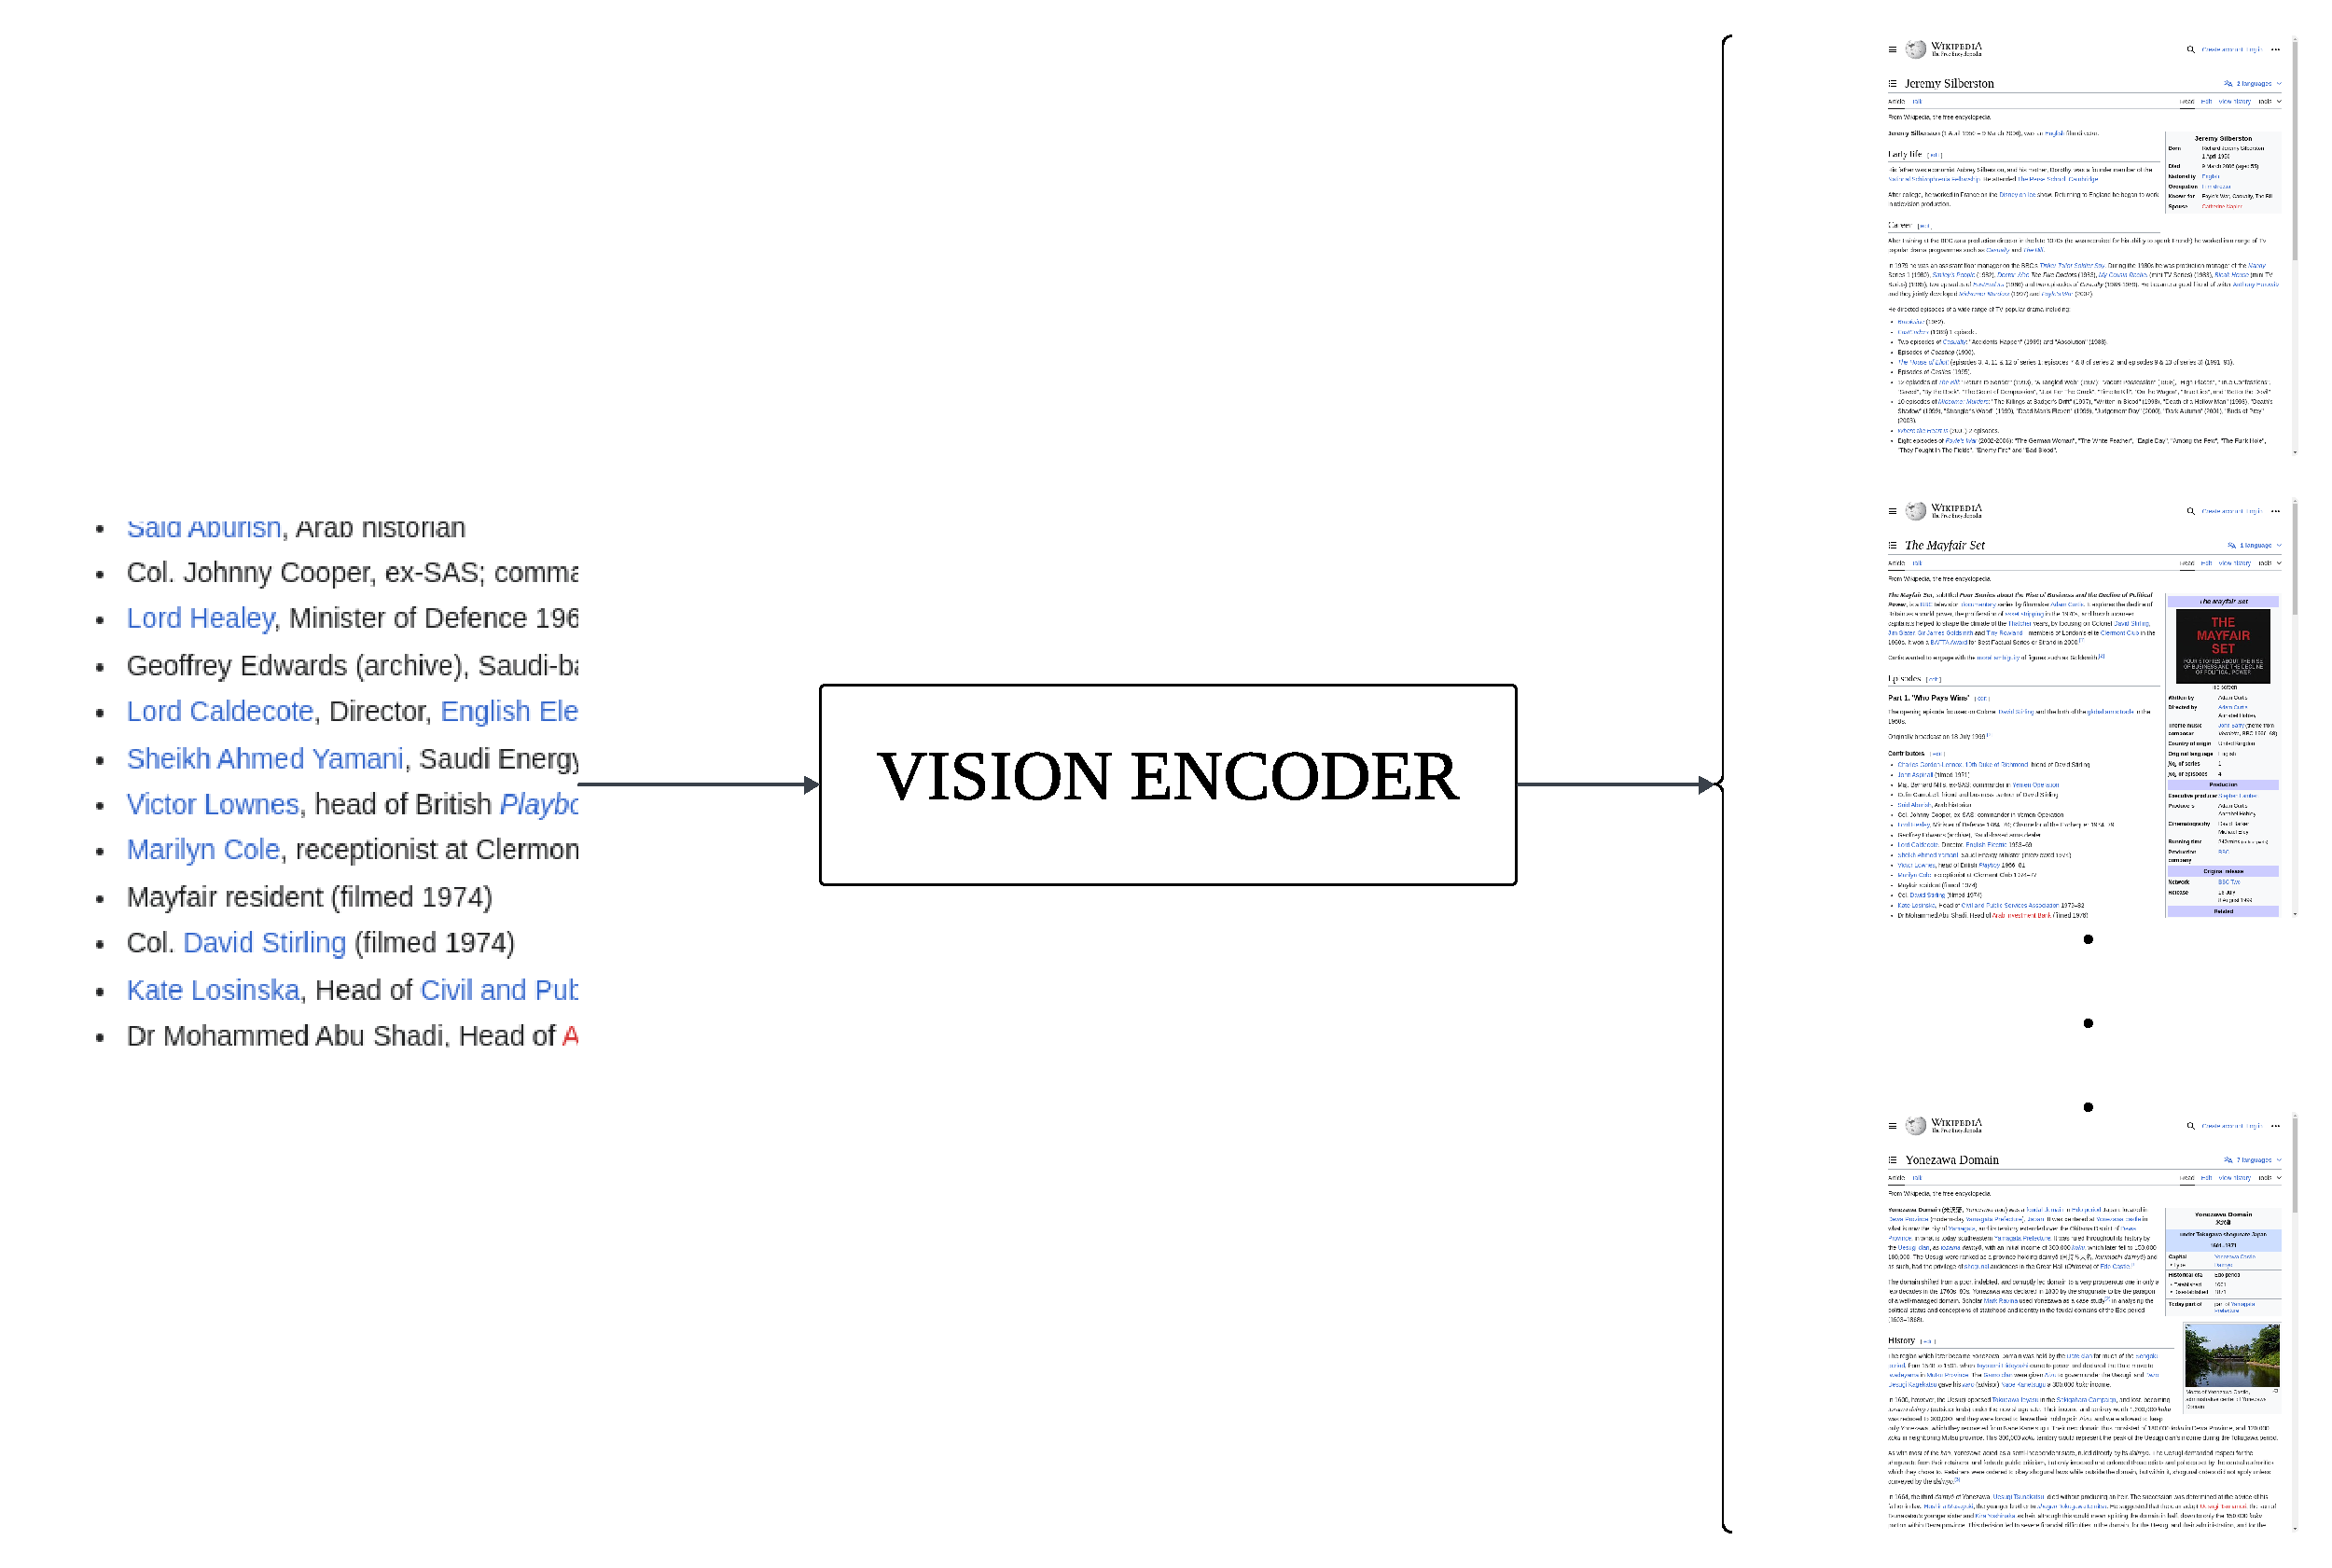
\includegraphics[width=\columnwidth]{figures/Benchmark.pdf}
\caption{Anchor-pool benchmark (Phase 2). Each anchor crop is
encoded with the vision encoder and ranked against a small pool
($\sim$7 images) of positives (other crops of the same page) and
hard negatives (crops of unrelated pages).}
\label{fig:bench}
\end{figure}

\subsection{Evaluation}
\label{sec:eval}

We evaluate on a held-out slice of $P=2\,000$ pages disjoint from
training, with two complementary protocols.

\textbf{Protocol A --- crop $\rightarrow$ page (headline metric).}
For each query crop $c$ on page $p$ with crops
$\{c_1,\dots,c_{n_p}\}$, the gallery vector for any page $q\neq p$
is the L2-normalised mean of all $q$'s crop embeddings. The
gallery vector for page $p$ is recomputed leaving the query out:
\(g_p^{\setminus c} = \mathrm{normalise}\!\bigl(\sum_i \phi(c_i) - \phi(c)\bigr)\).
We cosine-rank the $P$ gallery vectors against $\phi(c)$ and
report R@$k$ as the fraction of queries whose source page lands
in the top $k$. Random R@1 $=1/P=5\times 10^{-4}$. The
leave-one-out aggregation forbids the trivial
``find another crop of the same column'' shortcut implicit in
earlier crop-vs-crop formulations of this task.

\textbf{Protocol B --- anchor-pool transfer.} The anchor-pool
benchmark of Figure~\ref{fig:bench} uses 118 valid validation
triplets from \texttt{Wikipedia\_SS\_withanchors}. For each anchor
crop, the pool is the union of its positives and hard negatives
($\sim$7 images). We rank the pool by cosine similarity and
report R@1. This measures cross-set transfer: anchors and pool
images come from a different distribution of crops than what the
model trained on.

\subsection{Platonic alignment}
\label{sec:platonic}

For each (image encoder $E_v$, text encoder $E_t$) pair we encode
the same 2\,000-page eval slice with both halves: image features
$\mathbf{X} \in \mathbb{R}^{N\times d_v}$ from page screenshots,
text features $\mathbf{Y}\in\mathbb{R}^{N\times d_t}$ from page
titles. We report mutual-$k$NN at $k=10$ (the fraction of points
sharing at least one of their top-10 neighbours under the two
embeddings), debiased CKA \cite{kornblith2019cka, murphy2024align},
and Procrustes distance. The Platonic Hypothesis predicts a
positive rank correlation between $E_v$'s alignment and $E_v$'s
downstream cross-modal retrieval performance. We test this
directly in \S\ref{sec:results}.

\section{Results}
\label{sec:results}

\subsection{Zero-shot retrieval}

\begin{table}[t]
\caption{Protocol-A zero-shot retrieval at $P=2000$. Random R@1
$=5\times 10^{-4}$. Encoder rows are coloured by pretraining family:
\colorbox{cITC}{\strut\hspace{2pt}image--text contrastive\hspace{2pt}}\,
\colorbox{cSSL}{\strut\hspace{2pt}image-only self-supervised\hspace{2pt}}\,
\colorbox{cSUP}{\strut\hspace{2pt}supervised\hspace{2pt}}\,
\colorbox{cRND}{\strut\hspace{2pt}random\hspace{2pt}}.
``Gap'' is same-page minus diff-page mean cosine similarity.}
\label{tab:zeroshot}
\centering
\small
\begin{tabular}{lccccc}
\toprule
Encoder & R@1 & R@5 & R@10 & R@20 & gap \\
\midrule
\rowcolor{cITC} CLIP ViT-B/16    & \textbf{0.548} & 0.715 & \textbf{0.779} & 0.833 & $+0.205$ \\
\rowcolor{cITC} SigLIP ViT-B/16   & 0.348 & 0.541 & 0.624 & 0.703 & $+0.110$ \\
\rowcolor{cSSL} DINOv2 ViT-B/14   & 0.022 & 0.043 & 0.058 & 0.075 & $+0.010$ \\
\rowcolor{cSSL} I-JEPA ViT-H/14   & 0.002 & 0.008 & 0.015 & 0.021 & $-0.002$ \\
\rowcolor{cSUP} ImageNet ViT-B/16 & 0.009 & 0.022 & 0.031 & 0.043 & $-0.002$ \\
\rowcolor{cRND} Plain ViT-B/16     & 0.007 & 0.020 & 0.029 & 0.042 & $+0.000$ \\
\bottomrule
\end{tabular}
\end{table}

Table~\ref{tab:zeroshot} reports zero-shot Protocol-A. CLIP
dominates at R@10 $=$~0.779, SigLIP follows at 0.624, and the four
image-only encoders cluster near random (R@10 $=$~0.015--0.058).
Three observations follow:

(i) The largest gap is between the image--text contrastive and
the image-only families ($\Delta$R@10 $\approx 0.57$), not between
encoders within a family. The supervised ImageNet ViT scores 0.031
versus 0.029 for the random-init plain ViT, so ImageNet
classification supervision adds essentially nothing for this task.

(ii) I-JEPA scores R@10~$=$~0.015, \emph{below} the random-init
plain ViT (0.029). Despite ViT-H/14 being roughly 5$\times$ larger
than the ViT-B encoders, image-only predictive pretraining
out-of-the-box does not transfer to visual document retrieval.
Q2's optimistic reading is therefore falsified at the zero-shot
level: a post-hoc text adapter (\S\ref{sec:disc}) is the only
remaining path to rescue I-JEPA.

(iii) The CLIP--SigLIP gap (0.155) is real but small relative to
the CLIP--DINOv2 gap (0.721). The dominant predictor is whether
the encoder saw paired image--text data, not the specific
contrastive form (softmax vs.\ sigmoid).

\subsection{Fine-tuning}

\begin{table}[t]
\caption{Protocol-A retrieval after last-4-block fine-tuning, single
seed. ``$\Delta$ZS'' is R@10 minus the encoder's zero-shot baseline.
Yellow rows are fine-tuned variants of the encoder above them.}
\label{tab:finetune}
\centering
\small
\begin{tabular}{lccc}
\toprule
Encoder + head & R@1 & R@10 & $\Delta$ZS \\
\midrule
\rowcolor{cFT}  DINOv2 + MLP \,\,(30k)    & 0.351 & 0.787 & $+0.729$ \\
\rowcolor{cFT}  DINOv2 + SALAD (30k)      & 0.512 & 0.880 & $+0.822$ \\
\rowcolor{cFT}  DINOv2 + SALAD (50k)      & \textbf{0.569} & \textbf{0.915} & $+0.857$ \\
\rowcolor{cFT}  CLIP\, + SALAD\, (30k)     & 0.601 & 0.724 & $-0.055$ \\
\rowcolor{cFT}  CLIP\, + MLP\, (30k)$^\dagger$ & 0.000 & 0.000 & collapsed \\
\bottomrule
\multicolumn{4}{l}{\footnotesize $^\dagger$~Embeddings collapsed to
a constant.}
\end{tabular}
\end{table}

Table~\ref{tab:finetune} reports the fine-tuned grid.
DINOv2~+~SALAD on 30\,k pages reaches R@10~$=$~0.880 and on 50\,k
pages reaches 0.915, exceeding zero-shot CLIP (0.779). The MLP
head on the same DINOv2 backbone scores 0.787, so the SALAD
aggregator contributes $+9.3$\,pp R@10 over an MLP at the matched
backbone --- consistent with the prior place-recognition result of
\cite{izquierdo2024salad}.

CLIP fine-tuning at the conservative $\eta_{\text{bb}}=10^{-7}$
hurts more than it helps. CLIP+SALAD loses 5.5\,pp R@10 from its
own zero-shot baseline; the same-page minus diff-page sanity gap
shrinks from $+0.205$ to $+0.032$, indicating the fine-tune
sharpened the top-1 match (R@1 $+5.3$\,pp) but compressed the
overall similarity geometry. CLIP+MLP collapsed to a constant
output by step 400. Training CLIP at the LR that worked for
DINOv2 ($10^{-5}$) caused immediate divergence in earlier
attempts; $10^{-7}$ was chosen to avoid that, but evidently the
CLIP+MLP combination cannot navigate the resulting flat-loss
basin. A multi-LR sweep is the proper next step but is deferred.

\subsection{Platonic alignment predicts retrieval}

\begin{table}[t]
\caption{Mutual-$k$NN@10 between image and text encoders on the
same 2\,000-page eval slice. Bold = highest entry per row.
Row colours match Table~\ref{tab:zeroshot}.}
\label{tab:platonic}
\centering
\small
\begin{tabular}{lcccc}
\toprule
image $\backslash$ text & BERT & MiniLM & CLIP-T & SigLIP-T \\
\midrule
\rowcolor{cITC} CLIP             & 0.094 & 0.120 & \textbf{0.138} & 0.132 \\
\rowcolor{cITC} SigLIP           & 0.091 & 0.108 & 0.123 & \textbf{0.131} \\
\rowcolor{cSSL} DINOv2           & \textbf{0.027} & 0.021 & 0.019 & 0.026 \\
\rowcolor{cSSL} I-JEPA           & \textbf{0.019} & 0.014 & 0.016 & 0.018 \\
\rowcolor{cSUP} ImageNet ViT     & 0.018 & 0.013 & 0.013 & \textbf{0.019} \\
\rowcolor{cRND} Plain ViT (rand) & 0.008 & 0.007 & 0.007 & \textbf{0.009} \\
\bottomrule
\end{tabular}
\end{table}

\begin{figure}[t]
\centering
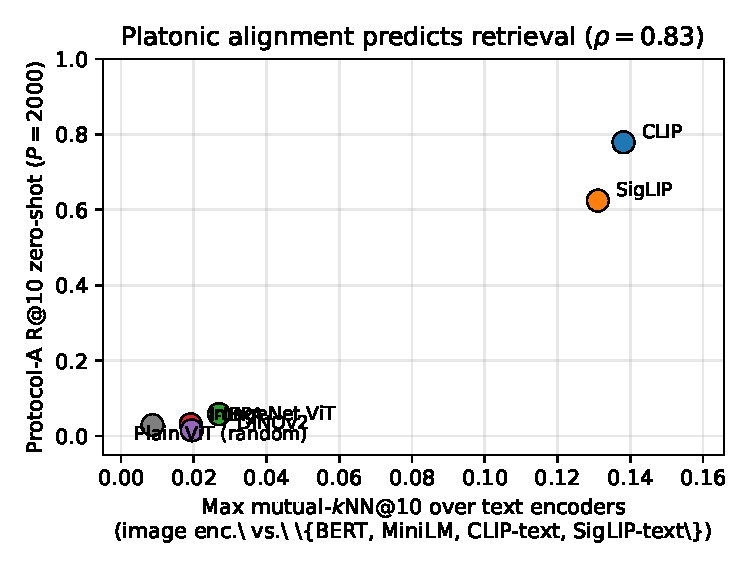
\includegraphics[width=0.95\columnwidth]{figures/platonic_vs_retrieval.pdf}
\caption{Each point is one image encoder. The $x$-axis is its
maximum mutual-$k$NN@10 against the four text encoders (column max
of Table~\ref{tab:platonic}); the $y$-axis is its zero-shot
Protocol-A R@10 (Table~\ref{tab:zeroshot}). Marker shape and pastel
colour code the pretraining family. Spearman $\rho = 0.83$
($p = 0.04$, $n = 6$).}
\label{fig:scatter}
\end{figure}

Table~\ref{tab:platonic} reports image-encoder $\times$
text-encoder mutual-$k$NN@10 alignment. CLIP and SigLIP align with
text encoders at 0.09--0.14; the four image-only encoders align at
0.007--0.027. Figure~\ref{fig:scatter} plots, for each image
encoder, its column-maximum text alignment against its zero-shot
Protocol-A R@10. The Spearman correlation is $0.83$ ($p=0.04$,
$n=6$): statistically significant even at this small sample size.
The two image--text contrastive encoders sit in the upper-right
corner; the four image-only encoders sit in the lower-left.

This is the central empirical claim of the paper. The kind of
pretraining the encoder received is a strong predictor of its
retrieval performance, mediated by its alignment with text
representations on the same content. The Platonic Hypothesis is
supported in this domain: encoders close to the text-encoder
geometry retrieve text-heavy visual documents better.

\subsection{Universal overspecialisation}

\begin{table}[t]
\caption{Phase-2 R@1 with the top fraction of every anchor and
pool image painted white. Every fine-tuned model improves under
blanking, indicating the model overweights the title-bearing top
region during fine-tuning. CLIP+MLP-30k figures are not informative
because the model collapsed.}
\label{tab:blank}
\centering
\small
\begin{tabular}{lccc}
\toprule
Run & orig.\ R@1 & b-15 R@1 & b-30 R@1 \\
\midrule
\rowcolor{cFT} DINOv2-MLP-30k     & 0.169 & 0.712 & 0.763 \\
\rowcolor{cFT} DINOv2-SALAD-30k   & 0.212 & 0.686 & 0.737 \\
\rowcolor{cFT} DINOv2-SALAD-50k   & 0.110 & 0.661 & 0.737 \\
\rowcolor{cFT} CLIP-SALAD-30k    & 0.551 & 0.686 & 0.720 \\
\rowcolor{cFT} CLIP-MLP-30k$^\dagger$ & 0.932 & 0.932 & 0.932 \\
\bottomrule
\multicolumn{4}{l}{\footnotesize $^\dagger$~Collapsed model;
embeddings are nearly identical.}
\end{tabular}
\end{table}

The original H-OCR test asks: ``does CLIP's R@1 drop when the
title is blanked?'' What we observe in Table~\ref{tab:blank} on the
trained checkpoints is the opposite. Every fine-tuned DINOv2 model
sees Phase-2 R@1 \emph{rise sharply} under blanking. The 50\,k
saturation checkpoint goes from R@1 $=$~0.110 (worse than DINOv2
zero-shot's 0.593) to 0.737 when the top 30\,\% of every test
image is painted white --- a $6.7\times$ improvement from
information removal. CLIP+SALAD shows the same trend in milder
form (0.551 $\to$ 0.720).

The mechanism is straightforward: fine-tuning on a single visual
corpus (Wikipedia screenshots) teaches the encoder that the
title-bearing top region perfectly identifies a page within the
training distribution, so it learns to overweight that region. On
in-distribution Protocol-A this is helpful (R@10 climbs with
training data). On the cross-set anchor pool, where positives and
hard negatives are crops sampled from arbitrary regions of unrelated
pages, the same overweighting becomes a confound. Removing those
pixels removes the confound and the underlying retrievable
features re-emerge. We did not anticipate this finding; it argues
for an explicit regularisation (e.g.\ random title-region masking
during training) as a future-work item.

\section{Discussion and Limitations}
\label{sec:disc}

\textbf{Single seed.} All training runs use one random seed. The
qualitative ordering across encoder families is large enough to
read past seed noise (the closest comparison, DINOv2-MLP-30k vs.\
DINOv2-SALAD-30k at $\Delta$R@10 $=0.093$, is well outside typical
single-seed jitter), but the within-family numbers (CLIP-SALAD vs.\
CLIP-MLP at the same LR) require multi-seed reruns before strong
claims.

\textbf{Pool size.} The headline retrieval pool ($P=2000$) is small
relative to industrial document corpora ($10^5$--$10^6$). The
Phase-2 pool ($\sim$7 candidates per anchor) is smaller still. Our
numbers should not be directly compared with ColPali-on-ViDoRe
\cite{faysse2025colpali}; the meaningful comparisons are
within-table between encoders evaluated on identical protocols.

\textbf{Crop resolution.} At $224\times 224$\,px input, body text is
sub-pixel. Anything called ``reading'' in this paper refers to
heading-level text and layout structure, not fluent body content.
A higher-resolution variant would change which signals are
available and is a natural follow-up.

\textbf{Direct H-OCR test.} The natural test of H-OCR for CLIP
zero-shot --- re-encode the eval slice with the title region
blanked, re-run Protocol-A --- requires a second descriptor cache
pass and is not in the present version. The trained-model
overspecialisation finding (Table~\ref{tab:blank}) is a partial
substitute but does not directly answer the H-OCR question for
zero-shot CLIP.

\textbf{I-JEPA + adapter.} Q2's most informative test is whether a
small linear adapter trained on (page-screenshot, page-title) pairs
can rescue I-JEPA to CLIP-level retrieval performance. We did not
run this experiment; it remains the cleanest way to test whether
text supervision is genuinely necessary or merely a shortcut.

\section{Conclusion}
\label{sec:conclusions}

We compared six image encoders trained with five distinct
pretraining objectives on a leak-free crop$\rightarrow$page
retrieval task over Wikipedia screenshots. Image--text contrastive
pretraining (CLIP, SigLIP) dominates zero-shot retrieval over
image-only self-supervision (DINOv2, I-JEPA), supervised
classification (ImageNet ViT), and random initialisation. Across
the six encoders, alignment with text encoders rank-correlates
with retrieval performance at Spearman $\rho = 0.83$, supporting
the Platonic Representation Hypothesis on this domain.
Fine-tuning DINOv2 with the SALAD aggregator on 50\,k pages
reaches R@10 $=$~0.915, exceeding zero-shot CLIP, but introduces a
universal pathology: the fine-tuned model overweights the title
region of every page, to the point that erasing those pixels at
test time improves cross-set transfer by up to $6.7\times$.

\bibliography{visword_report}
\bibliographystyle{comp547}

\end{document}
